\documentclass[]{beamer}
\usetheme{Singapore}
\usepackage{physics}
\usepackage[absolute,overlay]{textpos}
\usepackage{graphicx}
\usepackage{tikzit}

\setbeamertemplate{footline}[frame number]

\input{computation.tikzdefs}
\input{computation.tikzstyles}

\title{A novel notation for quantum cryptography}
\subtitle{Applications to some recent quantum cryptographic protocols and their equivalences}
\author{Zef Wolffs \\ External Research Supervisor: Boris Škorić \\ Internal Thesis Advisor: Jacco de Vries }

\expandafter\def\expandafter\insertshorttitle\expandafter{%
	\insertshorttitle\hfill%
	\insertframenumber\,/\,\inserttotalframenumber}

\begin{document}

\maketitle

\begin{frame}
\frametitle{Outline}

\begin{itemize}

\item Introduction
	\begin{itemize}
		\item Quantum Information
		\item Quantum Cryptography
		\item The Diagrammatic Notation
	\end{itemize}

\item The Classical One Time Pad
	\begin{itemize}
		\item Diagrammatic Implementation
	\end{itemize}

\item The Quantum One Time Pad
	\begin{itemize}
		\item Diagrammatic Implementation
		\item Equivalence: Quantum Teleportation
	\end{itemize}

\item Quantum Key Recycling
	\begin{itemize}
		\item Diagrammatic Implementation
		\item Equivalences
	\end{itemize}

\item Discussion and Conclusions

\end{itemize}
\end{frame}

\section{Introduction}

\begin{frame}
	\centering 
	\Huge
	\usebeamercolor[fg]{frametitle}{Introduction}
\end{frame}

\subsection{Quantum Information}

\begin{frame}
	\frametitle{Quantum Information}
	\begin{columns}
		\begin{column}{0.5\textwidth}
		\begin{itemize}
			\item The classical bit vs. the qubit
			\vspace{2cm}
			\item Mutual unbiasedness
		\end{itemize}
		\end{column}
		\begin{column}{0.5\textwidth}  %%<--- here
			\begin{center}
				\begin{textblock*}{10cm}(3cm,3cm)
				
\includegraphics[width=0.05\textwidth]{ClassicalBit.png}
				\end{textblock*}
				\begin{textblock*}{5cm}(8cm,2.6cm)
				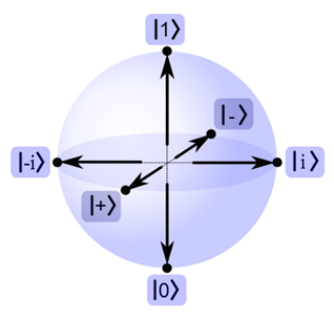
\includegraphics[width=0.5\textwidth]{QuantumBit.png}
				\end{textblock*}
				\begin{textblock*}{5cm}(7.1cm,5cm)
				\tiny	\textit{Representation of a classical bit (Left) and a qubit (right) \cite{Pomorski2018}.}
				\end{textblock*}
				\begin{textblock*}{7cm}(6.2cm,6cm)
					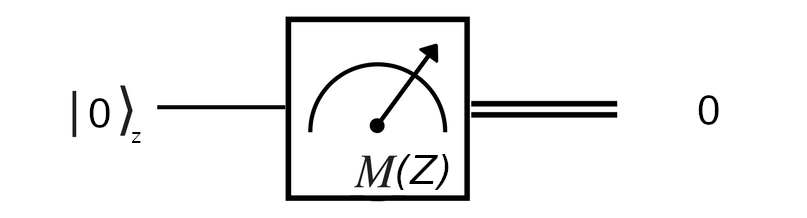
\includegraphics[width=0.5\textwidth]{MeasureInZ.png}
				\end{textblock*}
				\begin{textblock*}{7cm}(6.2cm,7cm)
				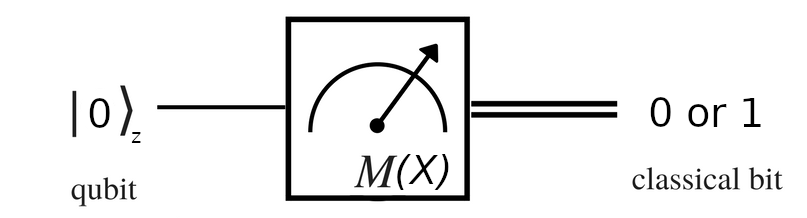
\includegraphics[width=0.5\textwidth]{MeasureInX.png}
				\end{textblock*}
				\begin{textblock*}{5cm}(7.2cm,8.1cm)
				\tiny	\textit{Measuring $\ket{0}_z$ in the Z and X bases \cite{Mishra2019}.}
				\end{textblock*}
			\end{center}
		\end{column}
	\end{columns}
\end{frame}

\subsection{Quantum Cryptography}

\begin{frame}
	\frametitle{Quantum Cryptography}
	\begin{columns}
		\begin{column}{0.6\textwidth}
				\begin{itemize}
				\item Quantum cryptographic protocols: Sending a message securely using quantum mechanics
				\vspace{2cm}
				\item Dirac notation is not very intuitive
				\end{itemize}
		\end{column}
	\begin{column}{0.5\textwidth}
		\begin{textblock*}{10cm}(7.4cm,2.8cm)
			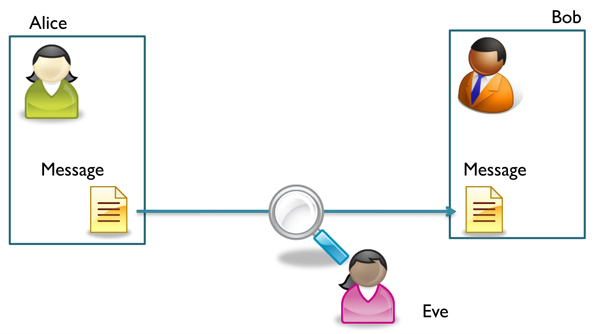
\includegraphics[width=0.5\textwidth]{AliceEveBob.png}
		\end{textblock*}
	\begin{textblock*}{6cm}(7.3cm,5.7cm)
		\tiny	\textit{Alice, Bob, and Eve's roles in (quantum) cryptographic protocols \cite{Cunche2011}.}
	\end{textblock*}
	\end{column}
	\end{columns}
\end{frame}

\subsection{The Diagrammatic Notation}

\begin{frame}
	\frametitle{The Diagrammatic Notation}
		\begin{textblock*}{12cm}(7cm,2.6cm)
		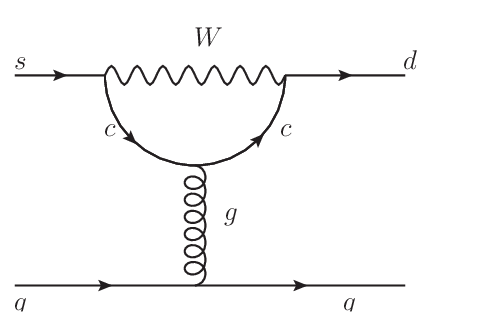
\includegraphics[width=0.5\textwidth]{PenguinDiagram.png}
	\end{textblock*}
	\begin{textblock*}{6cm}(1.6cm,6.9cm)
	\tiny	\textit{Diagrams in ecology: food webs \cite{Glaser}.}
	\end{textblock*}
	\begin{textblock*}{6cm}(7.2cm,6.9cm)
		\tiny	\textit{Diagrams in particle physics: Feynman diagrams \cite{Vos}.}
	\end{textblock*}
		\begin{textblock*}{12cm}(0.5cm,2.8cm)
		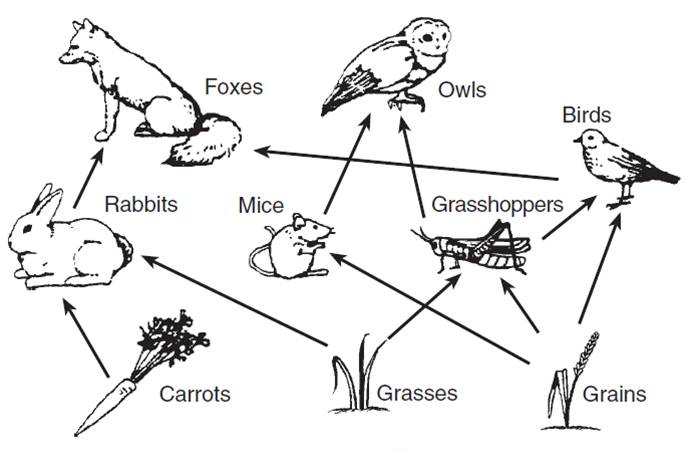
\includegraphics[width=0.5\textwidth]{FoodWeb.png}
	\end{textblock*}
\end{frame}

\begin{frame}
	\frametitle{The Diagrammatic Notation}
	\begin{itemize}
		\item Preparing a \textbf{classical bit} $\psi$ and \textbf{qubit} $\hat{\psi}$:
		\begin{equation}
		\tikzfig{state} ~~~~~~~~~ \tikzfig{thickSTATE}
		\end{equation}
		\item Applying a \textbf{classical map} $f$ and \textbf{quantum map} $\hat{f}$ to these states respectively:
		\begin{equation}
		\tikzfig{thinmap} ~~~~~~~~~ \tikzfig{thickMAP}
		\end{equation}
	\end{itemize}
\end{frame}

\begin{frame}
	\frametitle{The Diagrammatic Notation}
	\begin{itemize}
		\item \textbf{Spiders} copy states.
			\begin{equation}
			\tikzfig{thinSpiderCopy} = \tikzfig{thinSpiderCopy2} ~~~~~~ \tikzfig{SpiderCopy} = \tikzfig{SpiderCopy2}
			\end{equation}
		\item Whenever they have no input they create a random bit.
		\begin{equation}
		\tikzfig{Spideroneoutput} 
		\end{equation}
	\end{itemize}
\end{frame}

\section{The Classical One Time Pad}

\begin{frame}
	\frametitle{The Classical One Time Pad}
\end{frame}

\begin{frame}
	\frametitle{References}

	\bibliographystyle{plain}
	\bibliography{library}
\end{frame}

\end{document}